\chapter[Background]{Background}

\section{Graal Intermediate Representation (IR)}

The Graal IR \cite{Duboscq2013} models a program's structure and operations using a directed graph that represents both data and control flow between nodes. Each node in this graph is designed to produce at most a single value and follows the Static Single Assignment (SSA) \cite{Ron1991} form. Data flow is represented by input edges pointing upward to the operand nodes, control flow is depicted by successor edges pointing downwards to the successor nodes. 
In Graal IR, nodes are categorized as fixed or floating. Fixed nodes represent operations with strict execution order, such as control flow instructions, while floating nodes represent computations without fixed order constraints and can be freely reordered within the graph as long as dependencies are maintained. This flexibility allows the compiler during scheduling to reorder floating nodes to optimize execution. This IR framework provides a robust and efficient structure for code analysis and optimization, where optimization processes transform the graph to enhance overall performance. A critical aspect of this project is the conversion of the Graal IR into Prolog-compatible representations, enabling the optimizer to query and reason about the IR for potential optimizations. Consequently, a thorough understanding of the IR's structure and components is essential to accurately translate and utilize it within the Prolog-based optimization framework.

\begin{figure}[h]
    \centering
    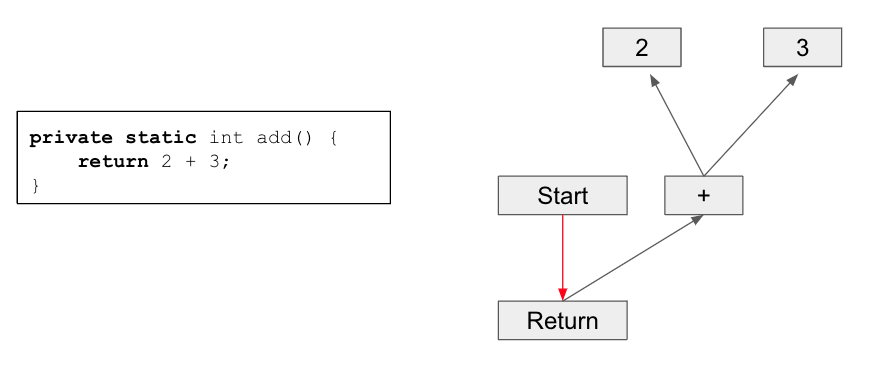
\includegraphics[width=0.5\textwidth]{Packages/graphir.png}
    \caption{Simple IR Graph}
    \label{figure:graphir}
\end{figure}

\autoref{figure:graphir} illustrates a simple IR graph corresponding to the Java code snippet below, with control flow edges highlighted in red. The graph starts at the Start node (node 0), which connects downward to an If node (node 9) that evaluates a condition based on node 6. Following data flow edges upward, this condition node compares parameter 1 (node 2) and constant 0 (node 5). The If node has two successors: the true branch on the left, beginning at node 8, and the false branch on the right, beginning at node 7. Each branch continues downward to Return nodes 11 and 13, respectively. Return node 11 produces its result by following data flow edges upward to node 10, which performs an addition operation, while Return node 13 follows data flow upward to node 12, which performs a subtraction. Both arithmetic nodes take parameter 1 (x) and parameter 2 (y) as the first and second operands. This traversal demonstrates how control and data flows interact to process and complete the function's execution.

\begin{lstlisting}[language=Java]
public int ifNode(int x, int y) {
    if (x == 0) {
        return x + y;
    }
    return x - y;
}
\end{lstlisting}


\section{GraalVM Compiler Optimizations}

In GraalVM, the compilation process is divided into two main phases. The first phase, involving the Graal IR, handles most of the high-level optimizations. This phase is further organized into three tiers: high-tier for high-level optimizations, mid-tier for memory-focused enhancements, and low-tier for low-level IR (LIR) conversion \cite{Graal2021}. This project primarily concentrates on high-tier optimizations within the GraalVM, specifically canonicalization rules for the \texttt{AddNode} and \texttt{AndNode}, as well as loop invariant reassociation optimizations, and conditional elimination.

Canonicalization is an essential early phase in the optimization process, focusing on transforming code into a standardized format and eliminating redundancies. This transformation simplifies and facilitates the application of subsequent optimizations. 
An example of canonicalization is shown in the code snippet below.
\begin{lstlisting}[language=Java]
// Before
return (x - y) + y;
// After
return x;
\end{lstlisting}

Loop invariant reassociation identifies expressions inside loops that yield the same result in every iteration and moves them outside the loop. This avoids repeated computation and reduces the loop's execution cost. It is a common technique for improving performance in tight computational loops. By reordering operands to group invariant values, the compiler can form a subexpression consisting entirely of invariants, represent it as a floating node, and hoist it outside the loop. An example of loop invariant reassociation is shown in the code snippet below.

\begin{lstlisting}[language=Java]
// Before
for (int i = 0; i < 1000; i++) {
    // inv1 and inv2 are invariant to the loop
    res = ((i + i) + inv1) + inv2;
}
// After
for (int i = 0; i < 1000; i++) {
    res = (i + i) + (inv1 + inv2);
}
\end{lstlisting}

Conditional elimination is an optimization that removes conditional branches that will never execute. This helps simplify control flow and reduce unnecessary branching in the program. By eliminating conditions that are always true or false, the resulting code is slightly more efficient and easier to optimize further. 
An example of conditional elimiation is shown in the code snippet below. The condition \(x == 2\) is always false, so the branch can be eliminated.
\begin{lstlisting}[language=Java]
// Before
if (x == 1) {
    if (x == 2) {}
}
// After
if (x == 1) {
}
\end{lstlisting}

\section{Prolog Programming Language}

In traditional imperative languages, a program consists of a sequence of instructions.
This approach emphasizes a step-by-step procedure where each instruction modifies the state of the machine to solve a given problem. 
In contrast, logic programming languages, such as Prolog, operate on a fundamentally different paradigm. 
Instead of prescribing a sequence of operations, logic programming focuses on defining a knowledge base composed of facts and rules \cite{Bramer2013}. After that, users can query the knowledge base to search for objects and relations. 

In Prolog, facts represent objects and their relationships, while rules specify the relationship between objects given it satisfies all the conditions. Once the knowledge base is established, users can formulate queries to extract information or solve problems by leveraging the logical relationships defined in the base using the depth-first search algorithm \cite{Chowdhary2020}. There may be several ways to achieve a given goal. The system initially selects the first available option. If Prolog fails to resolve a specific subgoal, it will backtrack to explore these previously noted alternatives. This mechanism, referred to as backtracking \cite{Chowdhary2020}, enables Prolog to systematically search for different solutions by revisiting and trying alternative paths.

\begin{figure}[h]
    \centering
    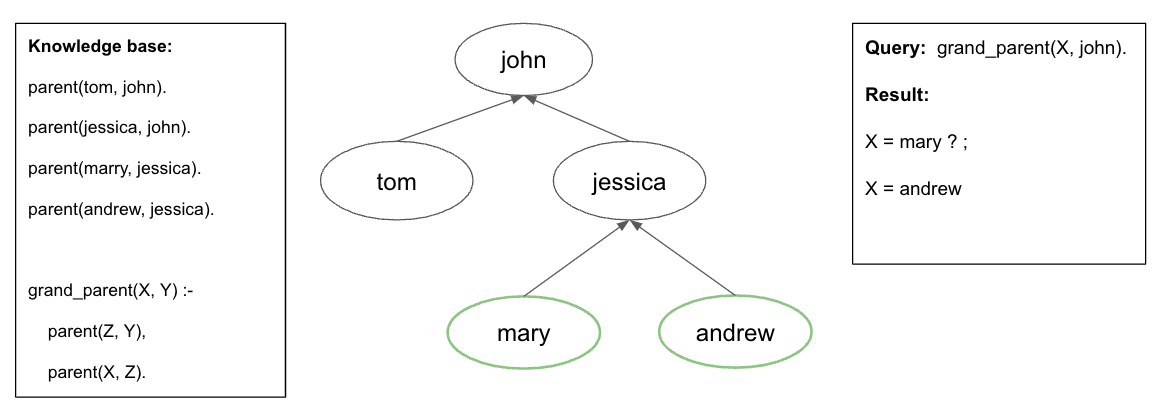
\includegraphics[width=0.9\textwidth]{Packages/Prolog.png}
    \caption{Example of Prolog specification}
    \label{figure:prolog}
\end{figure}

\autoref{figure:prolog} illustrates a Prolog program. The first three clauses are facts: john is a parent of tom and jessica, and jessica is a parent of both mary and andrew. The final clause is a rule defining the conditions for a grandparent relationship. When a query is made to determine the nodes for which john is a grandparent, Prolog performs a search from the first to the last clause, showcasing its backtracking behavior. Initially, Prolog identifies that john is a parent of tom, but since tom is not a parent of anyone, the search backtracks. It then considers the next option: jessica. Prolog then finds that jessica is a parent of mary. After exploring this path, Prolog backtracks again and continues to check the next possibility: jessica is also a parent of andrew, thereby completing the query.
In Prolog syntax, any atom or argument starting with a capital letter is treated as a variable, whereas atoms starting with a lowercase letter represent literal values or constants. This distinction is important for pattern matching and variable binding during query evaluation.
